\subsubsection{Inverse Reinforcement Learning}
\label{sec:irl}
The \textit{Inverse Reinforcement Learning} (IRL) problem, also known as \textit{Inverse Optimal Control}, is a LfD algorithm that addresses a significant challenge in Reinforcement Learning: designing an appropriate reward function for a given problem.

In many manipulation problems \cite{kalashnikov2018scalable}, using a binary and sparse reward function, where the reward is 1 if the task is completed correctly and 0 otherwise, can result in very long and inefficient training periods. For instance, in a reaching problem where the goal is to simply reach an object, the agent would receive a reward of 0 most of the time. More critically, actions that bring the agent closer to the object and actions that move it farther away would yield the same reward. In this simple example, a better reward function would measure the relative distance between the agent and the object. While this information can be easily obtained in simulations, it is often unavailable in real-world settings, forcing algorithm designers to make assumptions such as having prior knowledge about the object's location.

To address this issue, several research approaches have been proposed. One prominent approach is \textit{Reward Shaping}. In this method, the goal is to make the reward function more informative by introducing intermediate rewards during the agent's experience. These intermediate rewards are hand-engineered and require some degree of \textit{domain knowledge}.

The second approach, which is the focus of this chapter, is Inverse Reinforcement Learning (IRL). In IRL, the main idea is to \textbf{learn} the reward function $R$ which explains the expert behaviors contained in the dataset $\mathcal{D}^{E}$, and then use the learned $R$ to train the agent using classic RL algorithms.

The IRL procedure was introduced in \cite{abbeel2004apprenticeship}, and it is described by Algorithm \ref{alg:irl}. Essentially, the IRL algorithm is an iterative process where the parametrized reward function $R_{\omega}$ is first updated according to a given objective function $\mathcal{L}$. Subsequently, the updated reward function is used to update the learner's policy $\pi_{\theta}^{L}$.

\begin{algorithm}
\caption{Classic feature matching IRL algorithm}
\label{alg:irl}
\begin{algorithmic}
\Require Dataset of expert trajectories $\mathcal{D} = \left \{ \boldsymbol{\tau}^{E}_{i} \right \}^{N}_{i=1}$ 
\Require Reward function $R_{\omega}$, policy $\pi^{L}_{\theta}$ 
\While {policy improves}
    \State Evaluate the state-action visitation frequency $\mu$ of the current policy $\pi^{L}_{\theta}$
    \State Evaluate the objective function $\mathcal{L}$, w.r.t. $\mu$ and the dataset $\mathcal{D}$
    \State Update the reward-function parameters $\omega$ based on $\mathcal{L}$
    \State Update the policy $\pi^{L}_{\theta}$ through an RL algorithm, using the updated $R_{\omega}$
\EndWhile
\end{algorithmic}
\end{algorithm}

Generally speaking, the IRL approach faces two main challenges:
\begin{itemize}
    \item The learning process can be time-consuming and impractical for high-dimensional problems due to the double-nested optimization procedure.
    \item The IRL problem is \textit{ill-posed} because multiple reward functions can produce the same set of actions.
\end{itemize}

Despite these practical and theoretical challenges, various significant scientific contributions have been made in this field.

To solve the problem of multiple solutions for the reward function, constraints have been added to the optimization problem. Specifically, based on the type of constraint, there are two approaches:
\begin{enumerate}[label=\textbf{(\alph*)}]
    \item The \textit{Maximum Margin Prediction} (MMP) approach \cite{ratliff2006maximum_margin,ratliff2009learning_to_search}.
    \item The \textit{Maximum Entropy} (Max-Ent) approach \cite{ziebart2008maximum_entropy,wulfmeier2015deep_inverse_rl,finn2016guided_cost_learning}.
\end{enumerate}

The \textit{MMP} methods assume that the demonstrated trajectories are \textbf{optimal} and operate in a \textbf{deterministic} setting. The aim is to find the cost function such that the reward of the demonstrated trajectories, $R(\boldsymbol{\tau}^{E})$, is greater than the reward of all alternative trajectories, $R_{\omega}(\boldsymbol{\tau})$, by a certain margin $m$, solving the optimization problem formalized in Formula \ref{eq:mmp}.
\begin{equation}
\label{eq:mmp}
\underset{\omega, m}{\max} \ m \quad \text{s.t.} \quad R_{\omega}(\boldsymbol{\tau}^{E}) \geq \max (R_{\omega}(\boldsymbol{\tau})) + m
\end{equation}
The main problem with this formulation is that it does not handle the case in which the expert behavior is sub-optimal, leading to an ambiguous notion of margin.

In the \textit{Max-Ent} approach, the goal is to find the reward function parameters $\psi$ that drive the policy to maximize the entropy, subject to feature expectation matching (Formula \ref{eq:max_ent}).
\begin{equation}
    \label{eq:max_ent}
     \underset{\psi}{\max} \ \mathcal{H}(\pi^{r_{\psi}}) \quad \text{s.t.} \quad \mathbb{E}_{\pi^{r_{\psi}}}[\mathbf{f}] = \mathbb{E}_{\pi^{*}}[\mathbf{f}]
\end{equation}
The Max-Ent approach is the most popular in the IRL field since it removes the ambiguous aspects of the previous formulation. In the original work, the reward function was a linear combination of the features, i.e., $r_{\psi} = \psi^T \mathbf{f}$. However, this reward formulation is not suited for high-dimensional feature spaces, which may require the capability to model non-linear reward structures. In \cite{wulfmeier2015deep_inverse_rl}, a deep neural network was used to model the reward function. In this work, the neural network maps the feature vector $\mathbf{f}$ to the reward value and is trained according to the Maximum-Entropy setting. Experimental results have shown that the ability to approximate highly non-linear reward functions is essential for successfully solving tasks in high-dimensional discrete state spaces. A generalization to continuous state spaces was proposed in \cite{finn2016guided_cost_learning}. 

In particular, \cite{finn2016guided_cost_learning} addressed the problem of learning a cost function in a high-dimensional continuous state space with \textbf{unknown dynamics}. Starting from the exponential trajectory distribution $p(\tau) = \frac{1}{Z} \exp(-c_{\theta}(\tau))$,
the main difficulty is the estimation of the partition function $Z$, needed to compute the negative log-likelihood loss function (Formula \ref{eq:loss_reward_guided_cost_learning}).
\begin{equation}
    \label{eq:loss_reward_guided_cost_learning}
    \mathcal{L}_{\theta} = \frac{1}{N} \sum_{\tau^{E}_{i} \in D_{demo}} c_{\theta}(\tau^{E}_{i}) + \log(Z)
\end{equation}
Since the dynamics are unknown, the idea was to estimate the partition function through the trajectories obtained from the current policy rollouts, with the hypothesis that, during the learning of the cost function, the current policy drives the distribution towards regions where samples are more useful.

\begin{algorithm}[htbp]
\caption{Guided-Cost-Learning Algorithm \cite{finn2016guided_cost_learning}}
\label{alg:guided_cost_learning}
\begin{algorithmic}
\REQUIRE Initial controller $q_{k}(\tau)$ 
\FOR {i = 1, \dots, N}
    \STATE Generate $D_{traj}$ from $q_{k}(\tau)$
    \STATE $\mathcal{D}_{samp} \leftarrow \mathcal{D}_{samp} \bigcup \mathcal{D}_{traj}$
    \STATE Update the cost-function parameters, using $\mathcal{D}_{samp}$ and $\nabla_{\theta}\mathcal{L(\theta)}$
    \STATE Update the controller $q_{k+1}(\tau) \leftarrow q_{k}(\tau)$ according to \cite{levine2014lqr_flm} and using $\mathcal{D}_{traj}$
\ENDFOR
\end{algorithmic}
\end{algorithm}

Starting from these considerations, Algorithm \ref{alg:guided_cost_learning} was proposed. The algorithm returns a \textit{Linear-Quadratic Gaussian} \cite{levine2014lqr_flm} controller $q_{k}$, obtained by solving the problem in Formula \ref{eq:lqgc}.
\begin{equation}
    \label{eq:lqgc}
    \begin{aligned}
    q_{k} = \underset{q}{\arg \min} \ \mathbb{E}[c_{\theta}(\tau)] - \mathcal{H}(\tau) \quad \\ \text{s.t.} \quad p(s_{t+1}|s_{t},a_{t}) = \mathcal{N}(s_{t+1}; f_{x_t}x_{t}+f_{u_t}u_{t}, F_{t})
    \end{aligned}
\end{equation}

The cost function was parameterized according to a neural network, and experiments performed on real-robot manipulation tasks such as dish placement and pouring proved the effectiveness of the proposed method and the necessity of a non-linear representation of the cost function for complex problems, outperforming the classic Max-Ent method.

Recent methods have aimed to advance IRL towards more complex learning scenarios, such as learning a reward function from video demonstrations. In \cite{das2021model_based_irl_from_vd}, the architecture shown in Figure \ref{fig:model_based_irl} was proposed. The goal was to obtain the parameters $\Psi$ of a cost function $C_{\Psi}(\hat{\boldsymbol{\tau}}, z_{goal})$, enabling the derivation of a sequence of actions by minimizing the cost function itself (Formula \ref{eq:das2021model_based_irl_from_vd}).
\begin{equation}
\label{eq:das2021model_based_irl_from_vd}
\textbf{a}_{new} = \textbf{a} - \eta \nabla_{a} C_{\Psi}(\hat{\boldsymbol{\tau}}, z_{goal}).
\end{equation}
Different cost functions were proposed, all aiming to reduce the distance between the current predicted keypoints and the goal keypoint configuration. The trajectory $\hat{\boldsymbol{\tau}}$ is a sequence of predicted states $[\hat{s}_{1}, \dots, \hat{s}_{T}]$, resulting from a learned dynamic model, $\hat{s}_{t+1} = f_{dyn}(\hat{s}_{t}, a_{t})$. 

Experimental results demonstrated that it is possible to learn a cost function from human/robot video demonstrations. However, the proposed setting was tested on a very simple reaching task, highlighting that much work remains to be done to establish the effectiveness or ineffectiveness of IRL in complex real-robot manipulation tasks starting from video demonstrations.

\begin{figure}[th]
    \centering
    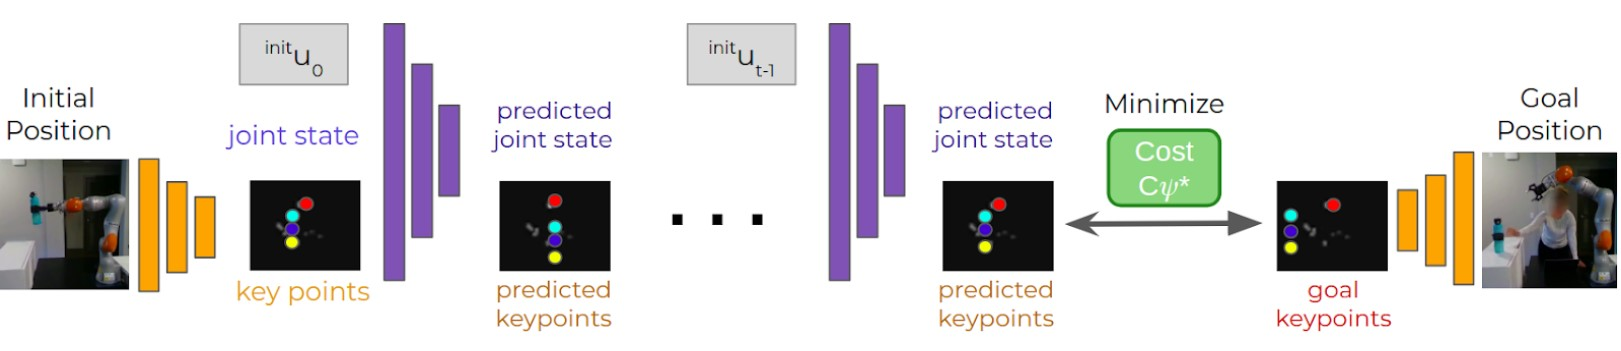
\includegraphics[width=\textwidth]{figures/images/model_based_irl/model_based_irl.jpg}
    \caption{Architecture proposed in~\cite{das2021model_based_irl_from_vd}.}
    \label{fig:model_based_irl}
\end{figure}
